\documentclass[landscape]{sciposter}

%\documentclass[a0, plainboxedsection, landscape]{sciposter}

\usepackage{multicol}
\usepackage{sectionbox}
\usepackage{graphicx}
\usepackage{subfig}
\usepackage{amsmath}
\usepackage{siunitx}
\usepackage{caption}
\usepackage[euler]{textgreek}

\renewcommand{\papertype}{custom}
%\renewcommand{\fontpointsize}{32 pt}
\setlength{\paperwidth}{48 in}
\setlength{\paperheight}{36 in}
\renewcommand{\setpspagesize}{
	\ifthenelse{\equal{\orientation}{landscape}}{
		\special{papersize=36 in, 48 in}
	}{\special{papersize=48 in, 36 in}
	}
}

\setmargins[4cm]
\leftlogo[0.7]{colby.jpg}
\norightlogo

\title{Millimeter-wave precision spectroscopy of potassium in Rydberg states}
\author{Huan Q. Bui, Charles Conover}
\institute{Department of Physics and Astronomy, Colby College, Waterville, Maine}
\conference{DAMOP - Milwaukee, Wisconsin - May 27 - 31, 2019}
%\sectionfont{\fontsize{32 pt}{40 pt}\selectfont}

\begin{document}
%\renewcommand{\titlesize}{\Huge}
\renewcommand{\titlesize}{\fontsize{50 pt}{70 pt}\selectfont}
\renewcommand{\authorsize}{\fontsize{32 pt}{40 pt}\selectfont}
\renewcommand{\instsize}{\fontsize{32 pt}{40 pt}\selectfont}
\maketitle

\fontsize{28 pt}{34 pt}\selectfont

\begin{multicols}{4}
\setlength{\columnseprule}{0pt}

\section*{Abstract}
{\normalfont We measure two-photon mm-wave transitions between nd$_j$ and (n+1)d$_j$ Rydberg states for 30 $\le$ n $\le$ 35 in $^{39}$K to an accuracy 5$\times$ 10$^{-8}$ to determine high-n d-state quantum defects and absolute energy levels. $^{39}$K atoms are trapped and cooled to 2-3 mK in a MOT, and excited from 4s$_{1/2}$ to nd$_{3/2}$ or nd$_{5/2}$ by frequency-stabilized 405 nm and 980 nm ECDL's in succession.  The magnetic-field insensitive nd$_j\rightarrow $ (n+1)d$_j$ $\Delta$m $=0$ transitions are driven by a 16 $\mu$s-long pulse of mm-waves before the atoms are selectively ionized for detection. The (n+1)d population is measured as a function of mm-wave frequency. Static electric fields in the MOT are nulled in three dimensions to eliminate DC Stark shifts. The transitions exhibit small but measurable AC Stark shifts at resonance. Field-free intervals are determined both by extrapolating a sequence of measurements made as a function of mm-wave power to zero and directly without extrapolation by applying Ramsey's separated oscillating fields method. Our results give quantum defects for the high-n states that are an order of magnitude more accurate than earlier measurements of these quantities.}

\begin{figure}
\begin{center}
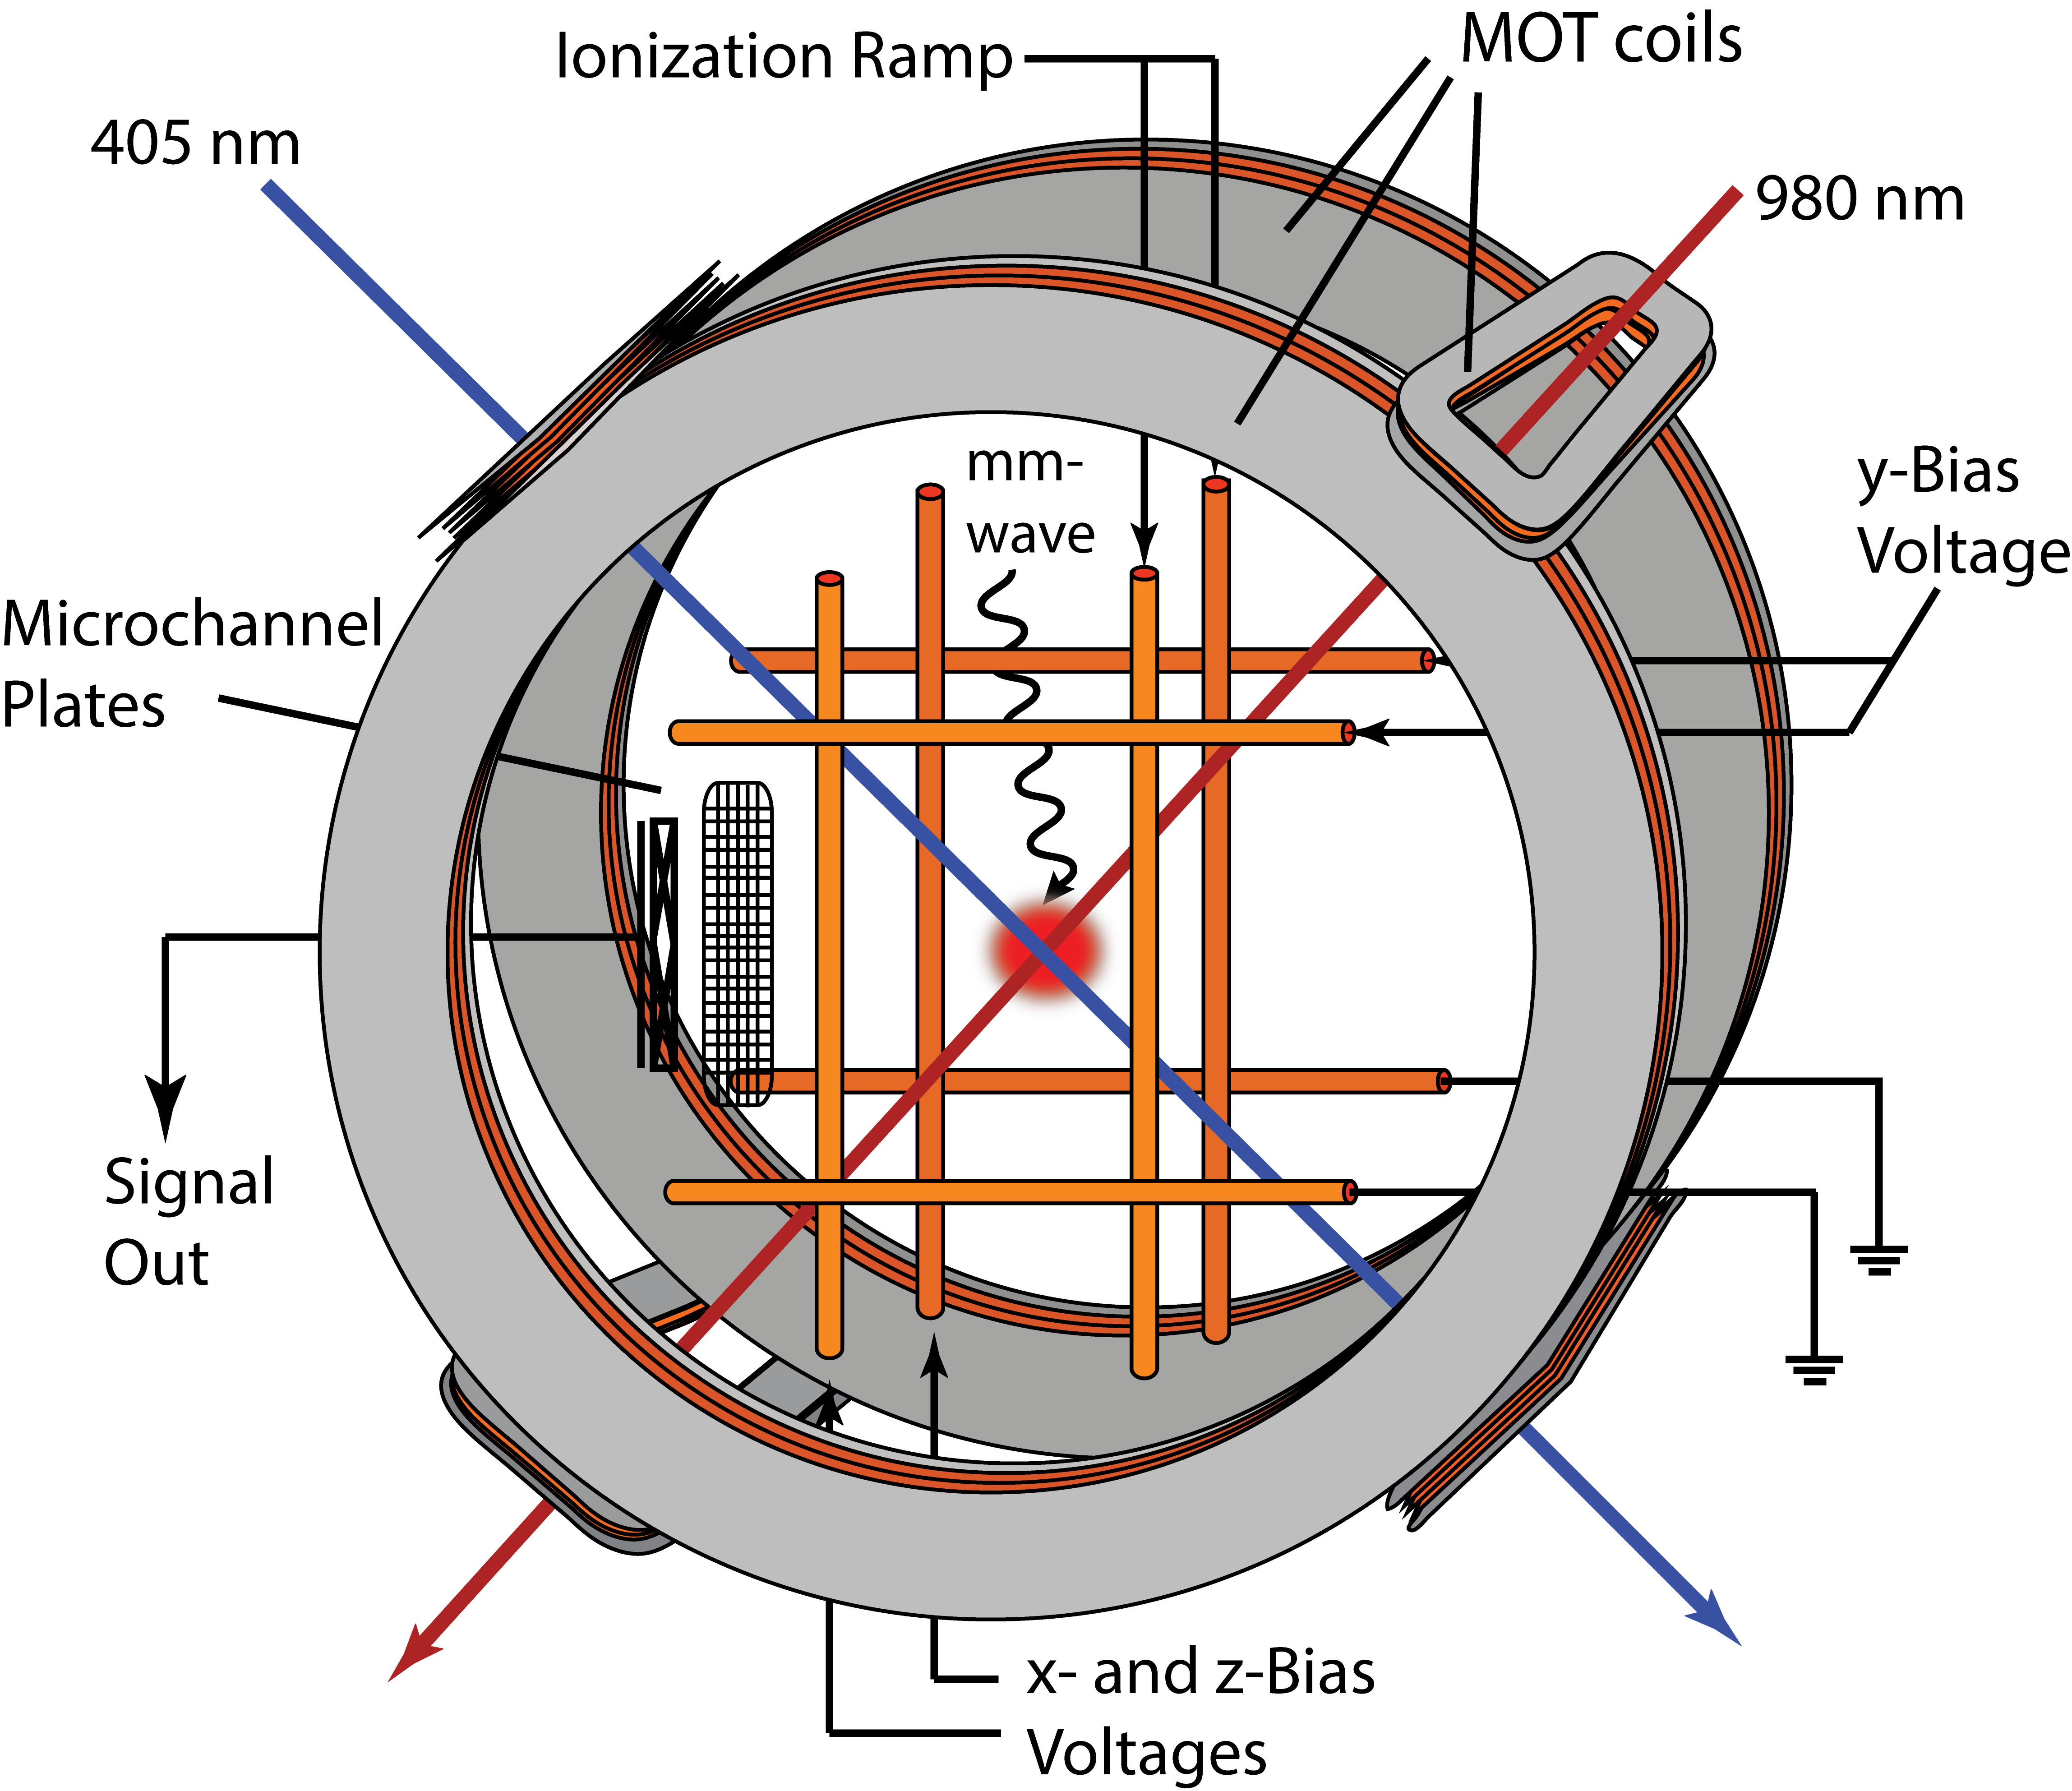
\includegraphics[scale = 0.65]{MOT.png}
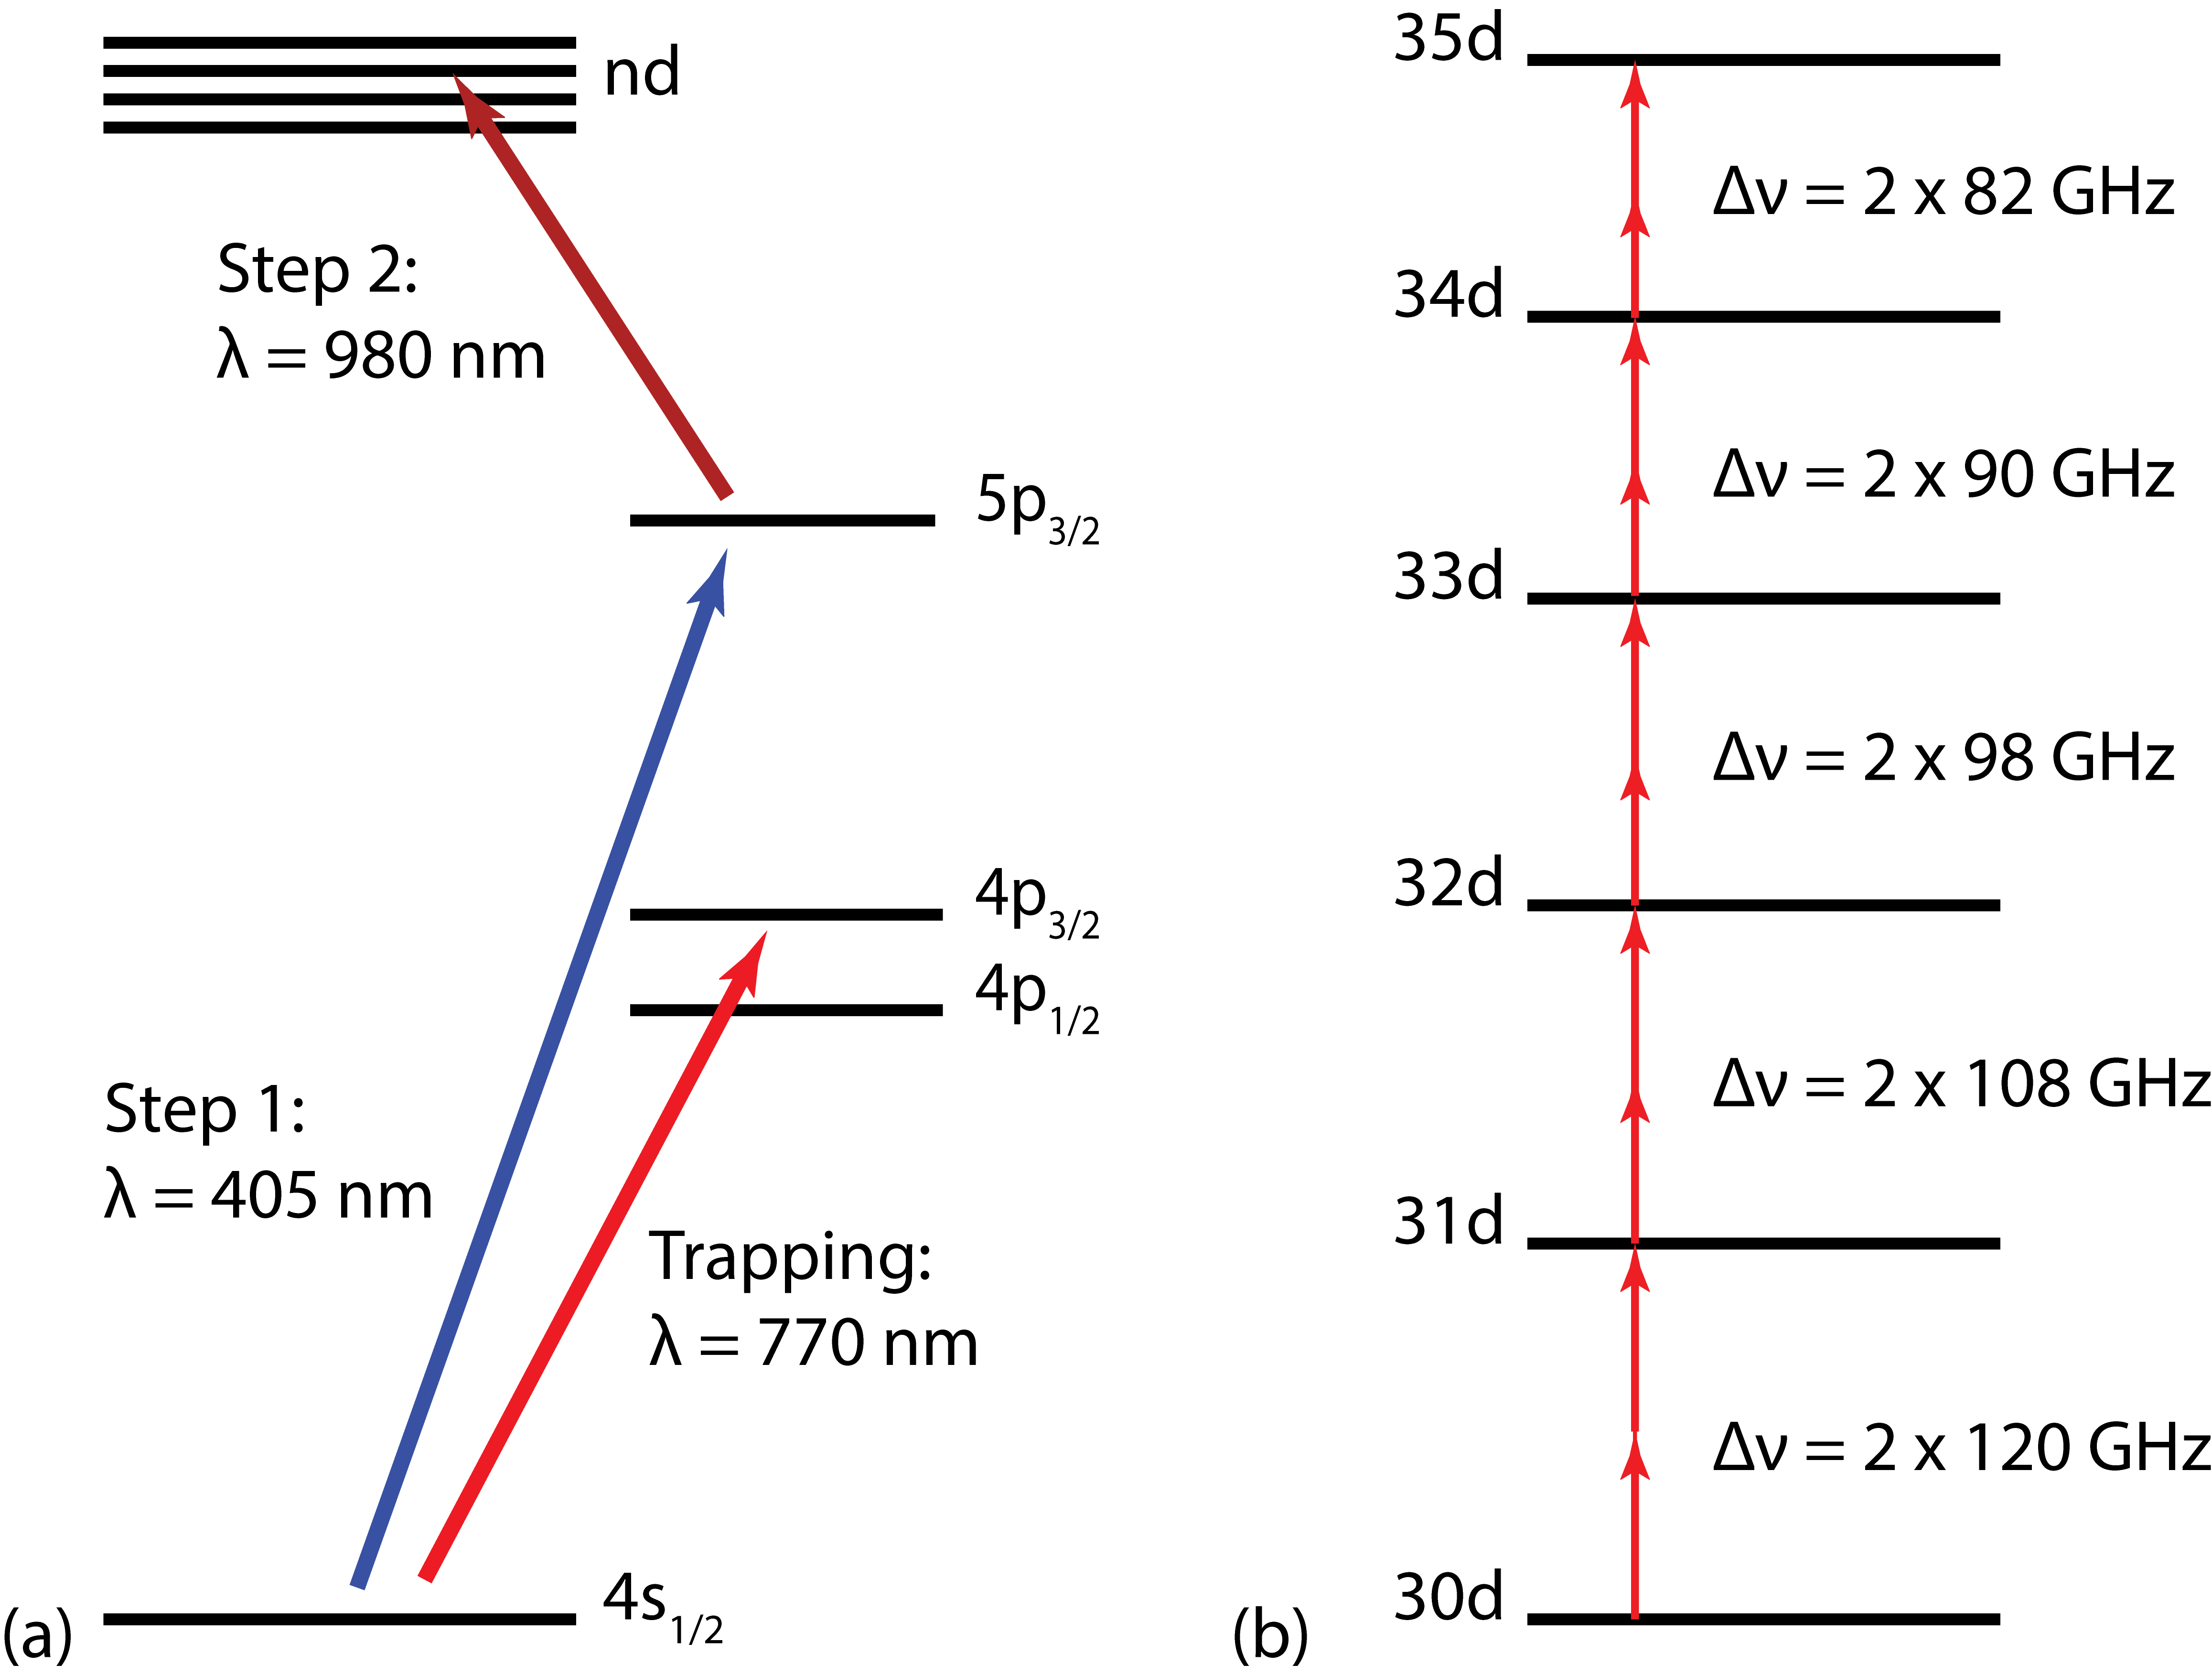
\includegraphics[scale = 0.65]{excitation.png}
%\normalfont{\caption{}}
%\label{Figure 1}
\end{center}
\end{figure}

\normalfont{The MOT cloud is trapped in a magnetic field and cooled by a 770 nm laser (not shown). The rods provide a static field and an ionization field. A mm-wave drives nd $\rightarrow$ (n+1)d transitions. (a) Trapping and excitations from 4s\textsubscript{1/2} to nd states in 2 steps. (b) Two-photon mm-wave transitions and their approximate frequencies.}

\section*{Magnetic-field insensitive $\mathbf{\Delta}$m = 0 transitions }
\begin{figure}
	\begin{center}
		\includegraphics[scale=0.75]{delta_m_0.eps}
	\end{center}
\end{figure}
\section*{Static field elimination}
Energy levels at highly excited states are sensitive to external static electric fields. Measured nd $\rightarrow$ (n+1)d transition frequencies vary quadratically with the static field amplitude:
{\Large $$\Delta \nu_{nd \rightarrow (n+1)d} = \nu_{0} - \frac{1}{2} \Delta \alpha E^2,$$}
where $\Delta \alpha$ is the difference between the (n+1)d and nd polarizabilities. In general, $\alpha$ represents how strongly energy levels shift in response to an external static electric field. 

\begin{figure}
\begin{center}
\includegraphics[scale = 0.65]{33d52_deltaV_population.eps}
\includegraphics[scale = 0.65]{33d52_DeltaV.eps}
\includegraphics[scale = 0.65]{33d52_Vy.eps}
\includegraphics[scale = 0.65]{33d52_VSum.eps}
%\caption{\normalfont{}}
%label{Figure 3}
\end{center}
\end{figure}

Static field elimination for 33d\textsubscript{5/2} $\rightarrow$ 34d\textsubscript{5/2} transition. Shown are 34d\textsubscript{5/2} population distributions and transition frequencies at different static field values in orthogonal directions. Projected maximum frequency in one direction corresponds to a DC bias that nullifies the field in that direction.

\section*{Zero mm-wave power extrapolation}
While not a large effect, the energy shift caused by the mm-wave source is significant at our level of precision. This shift is directly proportional to the intensity of the interacting mm-wave. 

\begin{figure}
\begin{center}
\includegraphics[scale = 0.8]{33d52_PScans.eps}
%\caption{\normalfont{}}
%\label{Figure 4}
\end{center}
\end{figure}

Zero-power extrapolation for 33d\textsubscript{5/2} $\rightarrow$ 34d\textsubscript{5/2} transition after static field elimination. The y-intercept of the linear fit of the measured transition frequencies is the mm-wave-free transition frequency. The energy shifts from 0.35 to 0 relative intensity are on the order of a few kHz.

\section*{Determination of d-state quantum defects}
The absolute energies are given by:
{\Large
$$E_n = -\frac{hcR_K}{(n - \delta(n))^2},$$}
where $n$ is the principal quantum number, and $\delta(n)$ is parameterized by two coefficients, $\delta_0$ and $\delta_2$, as:
{\Large
$$\delta(n) = \delta_0 + \frac{\delta_2}{(n-\delta_0)^2}.$$}

\begin{figure}
\begin{center}
\includegraphics[scale = 0.9]{d32_qd.eps}
\includegraphics[scale = 0.9]{d52_qd.eps}
%\caption{\normalfont{}}
%\label{Figure 5}
\end{center}
\end{figure}

nd $\rightarrow$ (n+1)d transition frequencies versus principal quantum number. A fit of the measured resonance frequencies are used to determine $\delta_0$ and $\delta_2$ for the d\textsubscript{3/2} and d\textsubscript{5/2} states. Residuals of the fit are less than a part in 10\textsuperscript{7} of the transition frequencies.

\section*{Ramsey's SOF, an alternative technique}
Ramsey's separated oscillatory field method removes the need for zero-power extrapolation. K atoms in the nd state are exposed to a double pulse of width $\tau$ and delay $T$ instead of a long, single pulse. 

\begin{figure}
\begin{center}
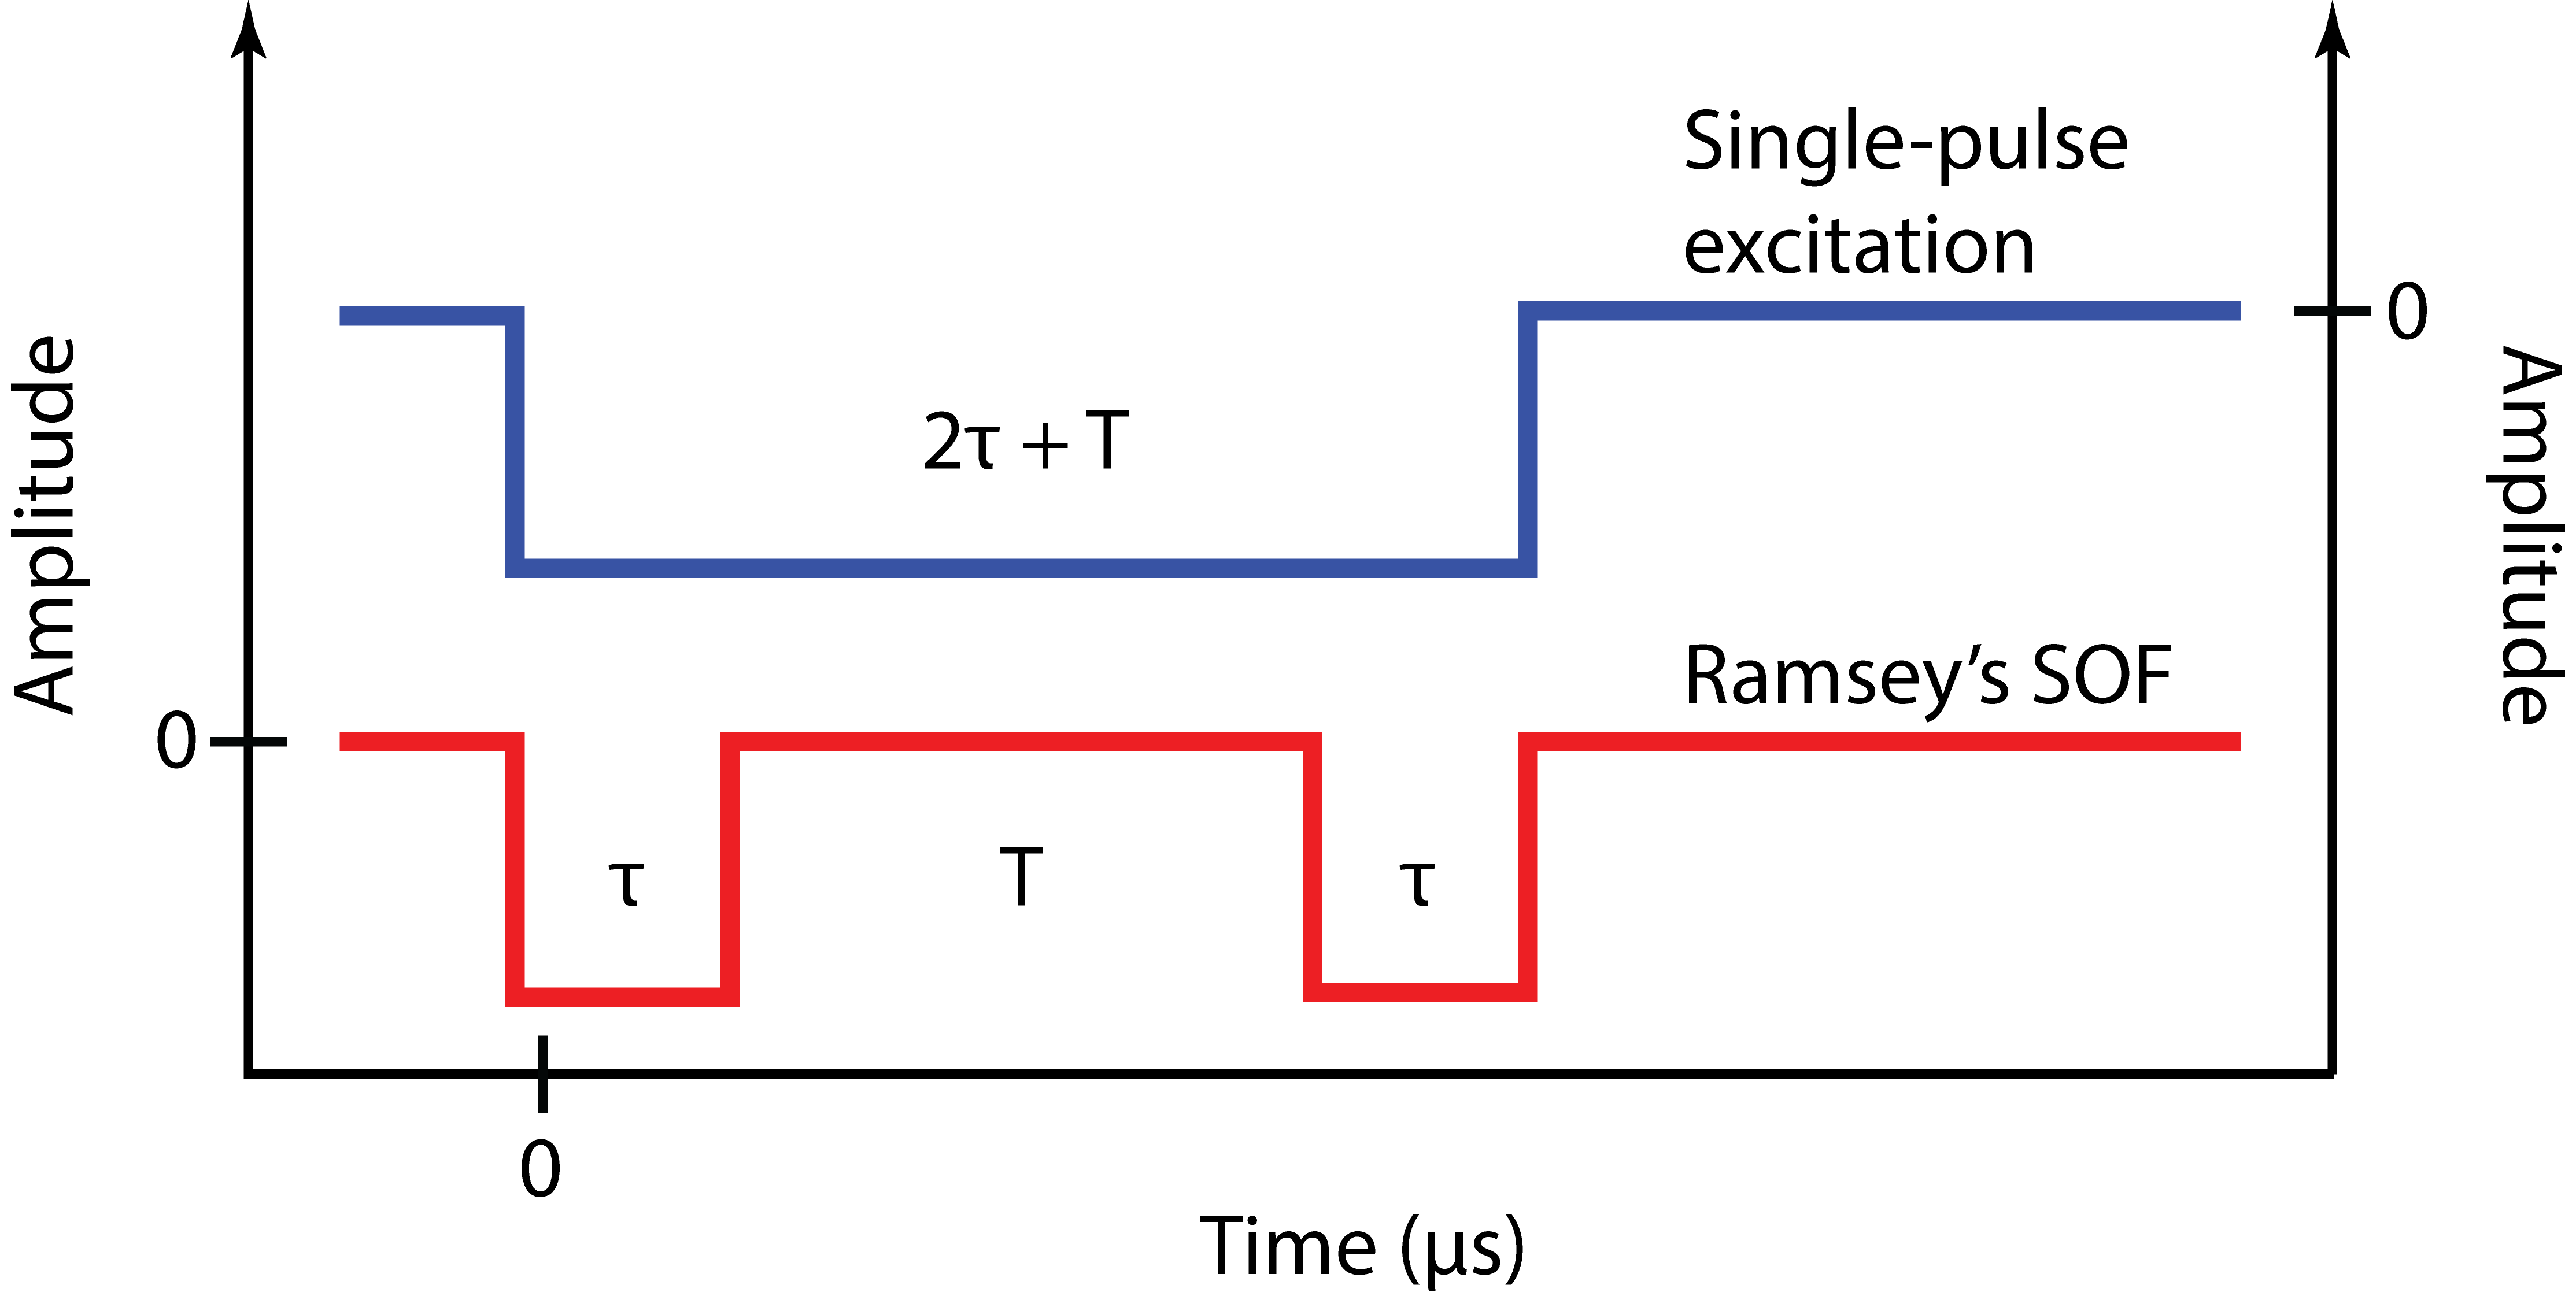
\includegraphics[scale=1]{Ramsey_excitation.png}
%\caption{\normalfont{}}
%\label{Figure 6}
\end{center}
\end{figure}
\begin{figure}
	\begin{center}
		\includegraphics[scale=1.5]{32d52_ramsey_1.eps}
		\includegraphics[scale=1.5]{32d52_ramsey_2.eps}
	\end{center}
\end{figure}
\noindent The final (n+1)d population oscillates as a function of $T$: 
{\Large
$$P_{(n+1)d} \propto {\cos}^{2}\left(\frac{\Delta_{0} T}{2}\right),$$}
where $\Delta_0=\omega_0-[E_{(n+1)d}-E_{nd}]/\hbar$ is the beat frequency between the mm-wave frequency and the atomic transition frequency in zero oscillatory field.
 
\begin{figure}
\begin{center}
\includegraphics[scale = 0.8]{33d52_delay_scans.eps}
%\caption{\normalfont{}}
%\label{Figure 7}
\end{center}
\end{figure}

With known mm-wave frequency offset, fitting a cosine squared to a delay scan signal allows for determining the zero-power frequency for the 33d\textsubscript{5/2} $\rightarrow$ 34d\textsubscript{5/2} transition.\\

The fit gives $\Delta_0/2\pi = \textrm{-0.4277 MHz}$. With an initial mm-wave frequency offset of $\textrm{-12.96 MHz}$, the field-free 33d\textsubscript{5/2} $\rightarrow$ 34d\textsubscript{5/2} spacing is:
\begin{align*}
\Delta \nu_0 &= \nu_{\textrm{offset}} - \Delta_0/2\pi + \textrm{179,496 MHz}\\
&= \textrm{-12.96 MHz + 0.4277 MHz + 179,496 MHz} \\ 
&= \textrm{179,483.47 MHz},
\end{align*}
consistent with the zero-power-extrapolated value.

\section*{Acknowledgments}
This research is supported by Colby College.

\end{multicols}

\end{document}
